\documentclass[a4paper]{article}
\usepackage[utf8]{vietnam}
\usepackage{scrextend}
\changefontsizes{13pt}
\usepackage{xcolor}
\usepackage{titlesec}
\usepackage{mdframed}
\usepackage{amsmath}
\usepackage{placeins}
\usepackage{array}
\usepackage[amsmath,standard,thmmarks]{ntheorem}
\usepackage{amssymb}
\usepackage{exscale}
\usepackage{amsfonts}
\usepackage{eucal}
\usepackage{enumerate}
\usepackage{enumitem}
\usepackage{commath}
\usepackage{graphicx}
\usepackage{tcolorbox}
\usepackage{url}
\usepackage[unicode]{hyperref}
\newmdenv[linecolor=black,skipabove=\topsep,skipbelow=\topsep,
leftmargin=-5pt,rightmargin=-5pt,
innerleftmargin=5pt,innerrightmargin=5pt]{mybox}
\setlength{\parindent}{0pt}
 \usepackage[left=2cm,right=2cm,top=2.5cm,bottom=2.5cm]{geometry}
\renewcommand{\baselinestretch}{1.5}
\newcommand{\heva}[1]{\left\{ 
\begin{aligned}#1\end{aligned}\right.}

\theoremstyle{nonumberplain} 
\theoremheaderfont{\itseries\slshape} 
\theorembodyfont{\normalfont}
\theoremsymbol{\ensuremath{_\blacksquare}} 
\renewtheorem{proof}{Chứng minh:}
\newcommand{\chm}[1]{\begin{proof}#1\end{proof}}

\usepackage{fancyhdr}
\pagestyle{fancy}
\fancyhf{}
\lhead{BTL2 - Mô hình hóa thống kê}
\cfoot{\thepage}
\rhead{Nhóm 4}
\title{BÀI TẬP LẦN 2 - MHHTK}

\allowdisplaybreaks

\author{NHÓM 4}

\date{\today}%

\begin{document}

\begin{titlepage}
\thispagestyle{empty}
\begin{center}
\textbf{\large{TRƯỜNG ĐẠI HỌC KHOA HỌC TỰ NHIÊN TP.HCM}\\
CAO HỌC KHÓA 30}\\
---------------*---------------
\end{center}
\vspace{0.3cm}
\begin{center}

\includegraphics[scale=0.8]{Logo-Math-CS.png} 
\end{center}
\vspace{0.7cm}
\begin{center}
\textbf{\Large{\textcolor[rgb]{1.0,0.0,0.0}{Bài tập lần 2}}}\\
\vspace{0.5cm}
\textbf{\Large{\textcolor[rgb]{1.0,0.0,0.0}{MÔ HÌNH HÓA THỐNG KÊ}}}\\
\vspace*{4cm}
$\begin{array}{rl}
\text{\large{Giảng viên hướng dẫn:}} &\text{\large{\bf TS. Nguyễn Thị Mộng Ngọc}}  \\
\vspace*{1cm}
\text{\large{Nhóm thực hiện:}}     & \text{\large{\textbf{Nhóm 4}}}
\end{array}$\\
\vspace{4cm}
\normalsize{TP. Hồ Chí Minh $-$ Tháng 01, 2021}
\end{center}
\end{titlepage}

\newpage
\thispagestyle{empty}
\begin{center}
\textbf{\large{BẢNG PHÂN CÔNG CÔNG VIỆC}\\}
\vspace{1cm}
\begin{tabular}{|m{3.7cm}||m{10cm}|m{1.8cm}|} 
\hline
\textbf{Thành viên} & \centering{\textbf{Công việc}} & \textbf{MSHV}\\
\hline
Đặng Khánh Thi & $-$ Bài 1: làm các ý 1, 2, 3, 4; kiếm tra các ý 5, 6, 7 & \\
& $-$ Bài 2: Làm các ý 4, 5, 6; kiểm tra các ý 1, 2, 3 & 20C29038 \\
& $-$ Bài 3: Làm các ý 1, 2, 3, 4, 5; kiểm tra các ý 6, 7, 8, 9, 10 & \\
& $-$ Kiểm tra và tổng hợp code R của bài 2 & \\
& $-$ Trình bày file bài tập & \\
\hline
Đinh Thị Nữ  & $-$ Bài 1: làm các ý  5, 6, 7; kiếm tra các ý 1, 2, 3, 4& \\
& $-$ Bài 2: Làm các ý 1, 2, 3; kiểm tra các ý 4, 5, 6 &  20C29013\\
& $-$ Bài 3: Làm các ý  6, 7, 8, 9, 10; kiểm tra các ý 1, 2, 3, 4, 5 & \\
\hline 
Lý Phi Long & $-$ Bài 1: làm các ý 1, 2, 3, 4; kiếm tra các ý 5, 6, 7 & \\
& $-$ Bài 2: Làm các ý 4, 5, 6; kiểm tra các ý 1, 2, 3 & 20C29028\\
& $-$ Bài 3: Làm các ý 1, 2, 3, 4, 5; kiểm tra các ý 6, 7, 8, 9, 10 & \\
& $-$ Kiểm tra và tổng hợp code R của bài 3 &\\
\hline
Phan Thị Thùy An & $-$ Bài 1: làm các ý  5, 6, 7; kiếm tra các ý 1, 2, 3, 4& \\
(Nhóm trưởng) & $-$ Bài 2: Làm các ý 1, 2, 3; kiểm tra các ý 4, 5, 6 & 20C29002 \\
& $-$ Bài 3: Làm các ý  6, 7, 8, 9, 10; kiểm tra các ý 1, 2, 3, 4, 5 & \\
& $-$ Kiểm tra và tổng hợp code R của bài 1 & \\
& $-$ Trình bày file bài tập & \\
\hline
\end{tabular}
\end{center}

\newpage
\section*{BÀI 1}
- $X_1$: áp lực công việc\\
- $X_2$: kỹ năng quản lý\\
- $X_3$: mức độ hài lòng với chức vụ của mình\\
- $Y$: mức độ lo lắng (biến phụ thuộc)
\begin{figure}[h!]
	\centering
	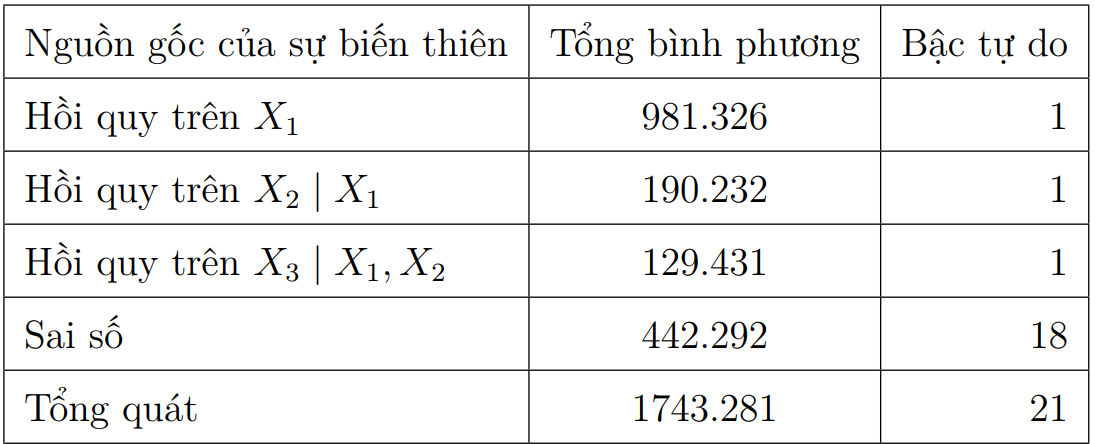
\includegraphics[scale =0.5]{anova1.PNG}  
	\caption{Bảng ANOVA bài 1}
	\label{ex1:model:1}
\end{figure}
\subsubsection*{1. Tính tổng bình phương hồi quy trên $X_1, X_2$ và $X_3$?}
$SSR = SSR_{X_1} + SSR_{X_2|X_1} + SSR_{X_3|X_1,X_2} = 981.326 + 190.232 + 129.431 = 1300.989$
\subsubsection*{2. Xác định tỷ lệ phần trăm sự biến thiên của mức độ lo lắng được giải thích bởi các biến độc lập.}

\[R^2 = \dfrac{SSR}{SST} = \dfrac{1299.989}{1743.281} = 0.7462876\]
Sự biến thiên của mức độ lo lắng được giải thích bởi các biến độc lập có tỉ lệ phần trăm là 74.63\%.

\subsubsection*{3. Có thể kết luận rằng trong tất cả ba biến giải thích đều có ảnh hưởng đáng kể đến mức độ lo lắng hay không? Chỉ rõ kiểm định nào được dùng.}

Đặt giả thuyết kiểm định:
\[\begin{cases}
	H_0: \beta_1 = \beta_2 = \beta_3 = 0\\
	H_1: \text{tồn tại ít nhất một } \beta_j \neq 0 \text{, với } j=1,2,3 
\end{cases}\]

Ta tính được giá trị thống kê Fisher:
\[F_{obs} = \dfrac{SSR/(p-1)}{SSE/(n-p)} = 17.64882\]

Với mức ý nghĩa $\alpha = 0.05$, tra bảng Fisher ta được:
\[F_{1-\alpha}(p-1,n-p) = F_{0.95}(3,18) = 3.16\]

Vì $F_{obs} > F_{0.95}(3,18)$ nên ta bác bỏ $H_0$ với mức ý nghĩa 5\%.

Vậy tồn tại \textbf{ít nhất} một trong ba biến áp lực công việc, kỹ năng quản lý, mức độ hài lòng với chức vụ của mình có ảnh hưởng đến mức độ lo lắng.

\subsubsection*{4. Nếu chúng ta chỉ xét biến giải thích $X_1$, hãy lập bảng ANOVA ?}

Khi chỉ xét $X_1$, mô hình hồi quy trở thành:
\[Y = \beta_0 + \beta_1X_1 + \epsilon\]

Vậy tổng sai số của biến giải thích $X_1$ là:
\[SSE_{X_1} = SST - SSR_{X_1} = 761.955\]

Với số mẫu $n=22$, ta lập được bảng ANOVA với biến giải thích $X_1$ như sau:

\begin{center}
	\begin{tabular}{|c|c|c|c|c|}
		\hline
		Biến thiên & SS & DF & MS & Fisher\\
		\hline
		$R_{X_1}$ & $SSR_{X_1} = 981.326$ & 1 &$SSR_{X_1}/1 = 981.326$ & \\
		\hline
		$E_{X_1}$ & $SSE_{X_1} = 761.955$ & $n-2 = 20$ & $SSE_{X_1}/20 = 38.09775$ & $MSR_{X_1}/MSE_{X_1} = 25.75811$\\
		\hline
		Total & 1743.281 & $n-1 = 21$ & & \\
		\hline
	\end{tabular}
\end{center}

\subsubsection*{5. Kiểm định giả thuyết sau với mức ý nghĩa 5\%}

\textbf{(a)} $H_0 : \beta_1 = 0$ \textbf{cho mô hình } $Y = \beta_0 + \beta_1 X_1 + \epsilon $ 

Đặt giả thuyết kiểm định:
\[\begin{cases}
	H_0 : \beta_1 = 0\\
	H_1 : \beta_1 \ne 0
\end{cases}\]

Thống kê của kiểm định: 
$$F =  \displaystyle \frac{MSR}{MSE} \sim F_{(1,20)} \text{ khi } H_0 \text{ đúng},$$ 
với $F_{(1,20)}$ là phân phối Fisher có bậc tự do 1 và 20.

Dựa vào bảng ANOVA ở câu 4, ta tính được giá trị thống kê:
$$F_{obs} = \displaystyle \frac{981.326}{38.09775} = 25.7581$$

Với mức ý nghĩa $\alpha = 0.05$, tra bảng Fisher ta được:
$$F_{1-\alpha}(1,n-2) = F_{0.95}(1,20) = 4.3512$$

Vì $F_{obs}>F_{0.95}(1,20)$ nên ta bác bỏ $H_0$ với mức ý nghĩa 5\%.

Vậy $Y$ được giải thích bởi một biến giải thích $X_1$.

\textbf{(b)} $H_0 : \beta_2 = 0$ \textbf{cho mô hình } $Y = \beta_0 + \beta_1 X_1 + \beta_2 X_2 + \epsilon $

Đặt giả thuyết kiểm định:
\[\begin{cases}
	H_0 : \beta_2 = 0 \text{ hay } Y = \beta_0 + \beta_1 X_1 + \epsilon \\
	H_1 : \beta_2 \ne 0 \text{ hay } Y = \beta_0 + \beta_1 X_1 + \beta_2 X_2 + \epsilon
\end{cases}\]

Thực hiện kiểm định Fisher từng phần, ta có thống kê của kiểm định: 
$$F = \displaystyle \frac{\left [ SSE (H_0) - SSE(H_1) \right ] / r}{SSE(H_1)/(n-p)} \sim F_{(r,n-p)} \text{ khi } H_0 \text{ đúng},$$
trong đó $r = 1, n = 22, p = 3$.

Trước tiên, ta cần tính $SSE (H_0)$ và $SSE(H_1)$:
$$SSE(H_0) = SST - SSR_{X_1} = 761.955 \text{, (đặt là } SSE_{X_1})$$
$$SSE(H_1) = SST - SSR_{X_1} - SSR_{X_2|X_1} = 571.723 \text{, (đặt là }  SSE_{X_1,X_2})$$

Giá trị thống kê $$F_{obs} = 6.3219$$

Với mức ý nghĩa $\alpha = 0.05$, tra bảng Fisher ta được:
$$F_{1-\alpha}(r,n-p) = F_{0.95}(1,19) = 4.3807$$

Vì $F_{obs}>F_{0.95}(1,19)$ nên ta bác bỏ $H_0$ với mức ý nghĩa 5\%.

Vậy $Y$ được giải thích bởi hai biến giải thích $X_1, X_2$.

\textbf{(c)} $H_0 : \beta_3 = 0$ \textbf{cho mô hình } $Y = \beta_0 + \beta_1 X_1 + \beta_2 X_2 + \beta_3 X_3 + \epsilon $

Đặt giả thuyết kiểm định:
\[\begin{cases}
	H_0 : \beta_3 = 0 \text{ hay } Y = \beta_0 + \beta_1 X_1 + \beta_2 X_2 + \epsilon \\
	H_1 : \beta_3 \ne 0 \text{ hay } Y = \beta_0 + \beta_1 X_1 + \beta_2 X_2 + \beta_3 X_3 + \epsilon 
\end{cases}\]
Thực hiện kiểm định Fisher từng phần, ta có thống kê của kiểm định: 

$$F = \displaystyle \frac{\left [ SSE (H_0) - SSE(H_1) \right ] / r}{SSE(H_1)/(n-p)}  \sim F_{(r,n-p)} \text{ khi } H_0 \text{ đúng},$$
trong đó $r = 1, n = 22, p = 4$.

Trước tiên, ta cần tính $SSE (H_0)$ và $SSE(H_1)$:
$$SSE(H_0) = SST - SSR_{X_1} - SSR_{X_2|X_1} = 571.723 \text{, (đặt là }  SSE_{X_1,X_2}) $$
$$SSE(H_1) = SST - SSR_{X_1} - SSR_{X_2|X_1} - SSR_{X_3|X_1,X_2} = 442.292 \text{, (đặt là }  SSE_{X_1,X_2,X_3})$$
Giá trị thống kê $$F_{obs} = 5.2675$$
Với mức ý nghĩa $\alpha = 0.05$, tra bảng Fisher ta được:
$$F_{1-\alpha}(r,n-p) = F_{0.95}(1,18) = 4.4138$$

Vì $F_{obs}>F_{0.95}(1,18)$ nên ta bác bỏ $H_0$ với mức ý nghĩa 5\%.

Vậy $Y$ được giải thích bởi cả ba biến giải thích $X_1, X_2$ và $X_3$.

\textbf{\underline{Kết luận cho câu 3}}

Vậy ta có thể kết luận rằng tất cả ba biến áp lực công việc, kỹ năng quản lý, mức độ hài lòng với chức vụ của mình \textbf{đều} có ảnh hưởng đến mức độ lo lắng của giám đốc.

\subsubsection*{6. Xác định hệ số xác định cho mỗi mô hình trong câu 5.}
\textbf{Mô hình 1:} $Y = \beta_0 + \beta_1 X_1 + \epsilon $ có hệ số xác định là
$$R^2_1 = 1 - \displaystyle \frac{SSE_{X_1}}{SST} = 0.5629$$


\textbf{Mô hình 2:} $Y = \beta_0 + \beta_1 X_1 + \beta_2 X_2 + \epsilon $ có hệ số xác định là
$$R^2_2 = 1 - \displaystyle \frac{SSE_{X_1,X_2}}{SST} = 0.6720$$
\textbf{Mô hình 3:} $Y = \beta_0 + \beta_1 X_1 + \beta_2 X_2 + \beta_3 X_3 + \epsilon $ có hệ số xác định là
$$R^2_3 = 1 - \displaystyle \frac{SSE_{X_1,X_2,X_3}}{SST} = 0.7463$$

\subsubsection*{7. Trong các mô hình trên, mô hình nào thích hợp nhất để giải thích sự biến động mức độ lo lắng của các giám đốc ?}
Để so sánh độ thích hợp của các mô hình có số lượng biến độc lập khác nhau, ta cần so sánh các hệ số xác định hiệu chỉnh theo công thức:
$$R^2_{adj} = 1 - \displaystyle \frac{SSE/(n-p)}{SST/(n-1)} \text{ với } n = 22$$
\textbf{Mô hình 1:} với $p=2$ ta có $${R^2_1}_{adj}  = 1 - \displaystyle \frac{SSE_{X_1}/20}{SST/21} = 0.5411$$ 

\textbf{Mô hình 2:} với $p=3$ ta có $${R^2_2}_{adj} = 1 - \displaystyle \frac{SSE_{X_1,X_2}/19}{SST/21} = 0.6375$$

\textbf{Mô hình 3:} với $p=4$ ta có $${R^2_3}_{adj} = 1 - \displaystyle \frac{SSE_{X_1,X_2,X_3}/18}{SST/21} = 0.7040$$

Dựa vào các giá trị $R^2$ hiệu chỉnh vừa tính, có thể kết luận \textbf{mô hình 3} là mô hình thích hợp nhất để giải thích sự biến động mức độ lo lắng của các giám đốc.
\newpage
\section*{BÀI 2}

\begin{figure}[h!]
	\centering
	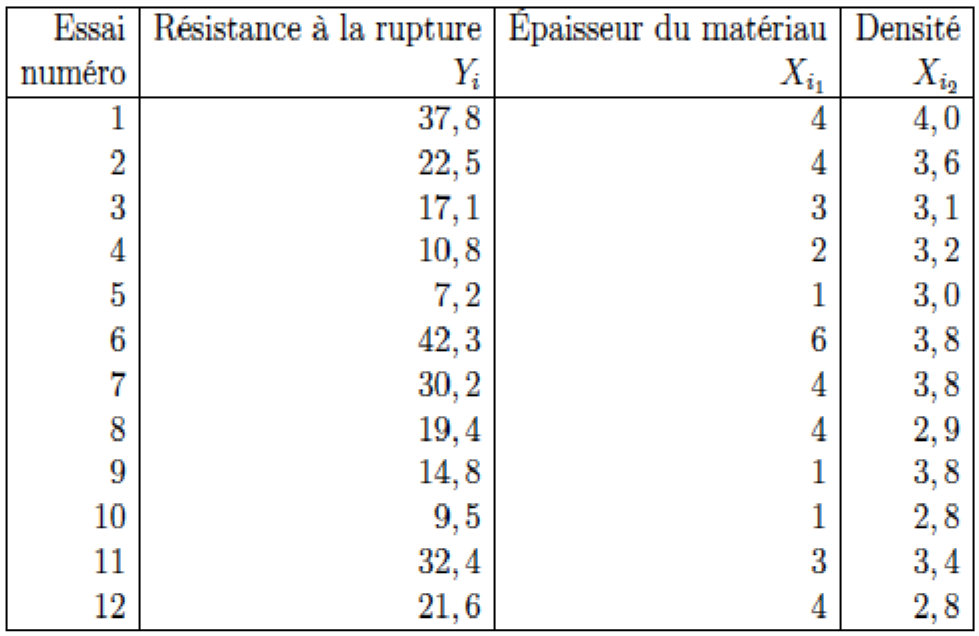
\includegraphics[width=0.6\linewidth]{bai-2-data}
	\caption{Bảng số liệu bài 2}
	\label{fig:bai-2-data}
\end{figure}

\begin{itemize}
	\renewcommand\labelitemi{--}
	\item $Y$: mức độ bền dẻo của nhựa
	\item $X_1$: độ dày của vật liệu
	\item $X_2$: mật độ của vật liệu
\end{itemize}

\subsubsection*{1. Tìm 2 phương trình đường thẳng hồi quy và 1 phương trình siêu phẳng (nếu có) ?}

Ta xây dựng các mô hình hồi quy như sau:

\textbf{Mô hình 1:} $Y= \beta_0 + \beta_1 X_1 + \epsilon$\\
Mô hình đường thẳng hồi quy tương ứng: $Y= \hat{\beta_0} + \hat{\beta_1} X_1$

\begin{figure}[h!]
	\centering
	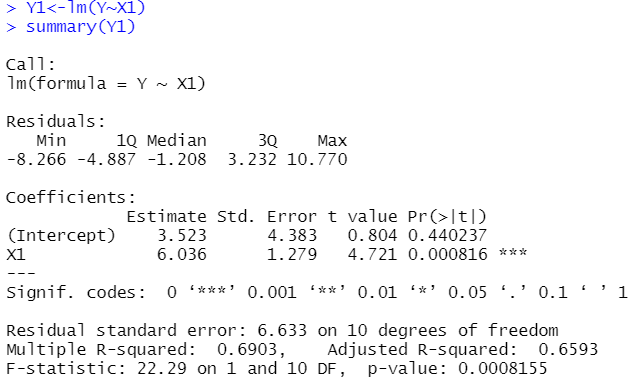
\includegraphics[scale =0.9]{bai2_1i.PNG}
	\caption{Tham số mô hình 1}
	\label{ex2:model:11}
\end{figure}

Dựa vào kết quả của phần mềm R ở hình \ref{ex2:model:11}, ta có $\hat{\beta_0} = 3.523$ và $\hat{\beta_1} = 6.036$, do đó ta có phương trình đường thẳng hồi quy theo độ dày của vật liệu ($X_1$) là:
\[Y = \hat{\beta_0} + \hat{\beta_1} X_1 = 3.523 + 6.036 X_1\]


\textbf{Mô hình 2:} $Y= \beta_0 + \beta_2 X_2 + \epsilon$\\
Mô hình đường thẳng hồi quy tương ứng: $Y= \hat{\beta_0} + \hat{\beta_2} X_2$

\begin{figure}[h!]
	\centering
	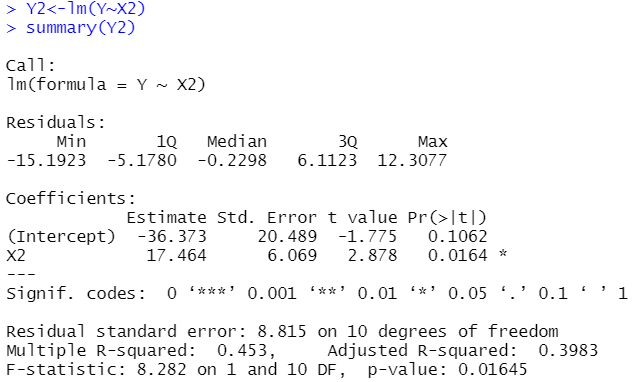
\includegraphics[scale =0.9]{bai2_1ii.PNG} 
	\caption{Tham số mô hình 2}
	\label{ex2:model:12}
\end{figure}

Dựa vào kết quả của phần mềm R ở hình \ref{ex2:model:12}, ta có $\hat{\beta_0} = -36.373$ và $\hat{\beta_2} = 17.464$, do đó ta có phương trình đường thẳng hồi quy theo mật độ của vật liệu ($X_2$) là:
\[Y = \hat{\beta_0} + \hat{\beta_2} X_2 = -36.373 + 17.464 X_2\]

\textbf{Mô hình 3:} $Y= \beta_0 + \beta_1 X_1 + \beta_2 X_2+ \epsilon$

Mô hình mặt phẳng hồi quy tương ứng: $Y= \hat{\beta_0} + \hat{\beta_1} X_1 + \hat{\beta_2} X_2$

\begin{figure}[h!]
	\centering
	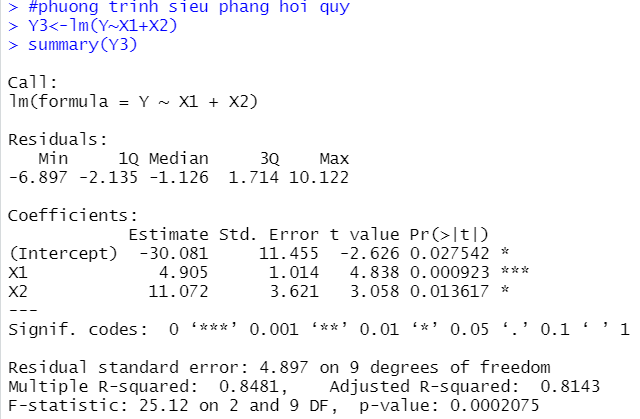
\includegraphics[width=0.7\linewidth]{bai2_1iii.PNG} 
	\caption{Tham số mô hình 3}
	\label{ex2:model:13}
\end{figure}

Dựa vào kết quả của phần mềm R ở hình \ref{ex2:model:13}, ta có $\hat{\beta_0} = -30.081$, $\hat{\beta_1} = 4.905$ và $\hat{\beta_2} = 11.072$, do đó ta có phương trình mặt phẳng hồi quy theo độ dày của vật liệu ($X_1$) và mật độ của vật liệu ($X_2$) là:
\[Y = \hat{\beta_0} + \hat{\beta_1} X_1 + \hat{\beta_2} X_2 = -30.081 + 4.905 X_1 + 11.072 X_2\]

\subsubsection*{2. Xác định tỷ lệ phần trăm sự biến thiên của biến phụ thuộc cho từng mô hình có thể có trên.}

\textbf{Mô hình 1:} Dựa vào kết quả mô hình 1 (hình \ref{ex2:model:11}), hệ số xác định $R^2= 0.6903$ cho biết có 69.03\% sự thay đổi của mức độ bền dẻo của nhựa được giải thích bởi độ dày của vật liệu ($X_1$).

\textbf{Mô hình 2:} Dựa vào kết quả mô hình 2 (hình \ref{ex2:model:12}), hệ số xác định $R^2= 0.453$ cho biết có 45.3\% sự thay đổi của mức độ bền dẻo của nhựa được giải thích bởi mật độ của vật liệu ($X_2$).

\textbf{Mô hình 3:} Dựa vào kết quả mô hình 3 (hình \ref{ex2:model:13}), hệ số xác định $R^2= 0,8481$ cho biết có 84.81\% sự thay đổi của mức độ bền dẻo của nhựa được giải thích bởi hai yếu tố là độ dày vật liệu ($X_1$) và mật độ của vật liệu ($X_2$).

\subsubsection*{3. Nếu chúng ta chỉ quan tâm đến cả 2 biến giải thích, hãy lập bảng ANOVA?}
\begin{figure}[h!]
	\centering
	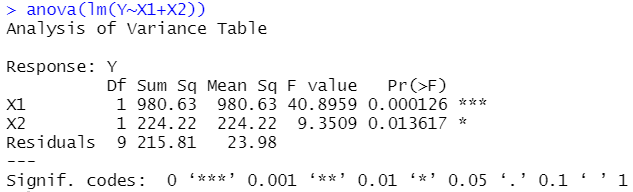
\includegraphics[width=0.7\linewidth]{bai2_3.PNG}
	\caption{Bảng ANOVA cho hai biến $X_1,X_2$}
	\label{ex2:model:anova3}
\end{figure}

Bảng ANOVA cho cả hai biến giải thích:
\begin{center}
	\begin{tabular}{|c|c|c|c|c|}
		\hline
		Biến thiên & SS & DF & MS & Fisher\\
		\hline
		$R_{X_1,X_2}$ & $SSR = 980.63+224.22 = 1204.85$ & 2 &$SSR/2 = 602.425$ & $MSR/MSE $\\
		\hline
		$E$ & $SSE = 215.81$ & $n-3 = 9$ & $SSE/9 = 23.9789$ & $= 25.123 $\\
		\hline
		Total & 980.63+224.22+215.81 = 1420.66& $n-1 = 11$ & & \\
		\hline
	\end{tabular}
\end{center}


\subsubsection*{4. Kiểm định giả thuyết sau với mức ý nghĩa 5\%}
Đặt giả thuyết kiểm định:
\[\begin{cases}
	H_0 : \beta_1 = \beta_2 = 0 \\
	H_1: \beta_j \neq 0 \text{ với } j=1,2 
\end{cases}\]

\begin{figure}[h!]
	\centering
	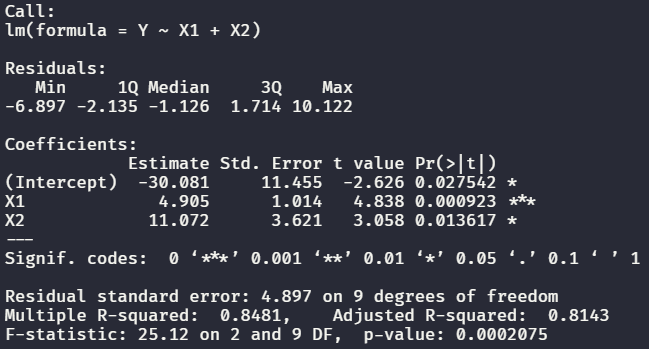
\includegraphics[width=0.7\linewidth]{bai-2-4-summary}
	\label{fig:bai-2-4-summary}
\end{figure}

Từ hình trên, ta có giá trị thống kê Fisher $F_{obs} = 25.12 \sim F_{0,95}(2,9)$, tính được $p\_value = 0.0002075386$ qua hàm \textbf{pf}:
\begin{figure}[h!]
	\centering
	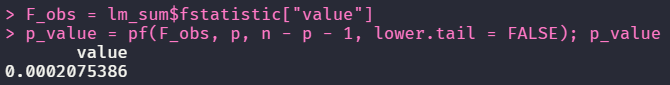
\includegraphics[width=0.7\linewidth]{bai-2-4-p_value}
	\label{fig:bai-2-4-pvalue}
\end{figure}

Vì $p\_value = 0.0002075386 < \alpha = 0.05$, suy ra bác bỏ giả thiết $H_0$.

\subsubsection*{5. Xác định khoảng tin cậy với mức ý nghĩa 5\% cho $\beta_1$ trong trường hợp mô hình chỉ có biến độc lập là độ dày của vật liệu ($X_1$).}

\begin{figure}[h!]
	\centering
	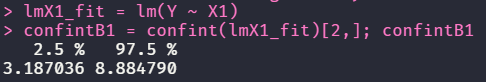
\includegraphics[width=0.7\linewidth]{bai-2-5-confint-beta1}
	\label{fig:bai-2-5-confint-beta1}
\end{figure}

Với độ tin cậy 95\%, khoảng tin cậy $\beta_1$ của mô hình có một biến độc lập $X_1$ là $[3.187036,8.88479]$.

\subsubsection*{6. Với khoảng tin cậy vừa tìm được ở câu 5, chúng ta có thể khẳng định rằng hồi quy tuyến tính là có ý nghĩa giữa mức độ bền dẻo của nhựa và độ dày của vật liệu và mật độ của vật liệu không? Chứng minh điều khẳng định của bạn.}

Nếu chỉ dựa vào khoảng tin cậy của $\beta_1$ ở câu 5, chúng ta \textbf{không} thể khẳng định được điều trên, vì kết quả ở câu 5 chỉ cho ta biết mối quan hệ tuyến tính giữa mức độ bền dẻo ($Y$) với độ dày của vật liệu ($X_1$).

Để chứng minh, ta lần lượt thực hiện kiểm định các giả thuyết sau:
\begin{enumerate}
	\item[i)] $H_0 : \beta_1 = \beta_2 = 0$ cho mô hình $Y = \beta_0 + \beta_1 X_1 + \beta_2 X_2 + \epsilon $
	
	Đặt giả thuyết kiểm định:
	\[\begin{cases}
		H_0 : \beta_1 = \beta_2 = 0 \\
		H_1: \beta_j \neq 0 \text{ với } j=1,2 
	\end{cases}\]

	Với kết quả từ câu 4, $H_0$ bị bác bỏ do chứng minh trên, nghĩa là tồn tại tham số $\beta_1$ hoặc $\beta_2$ trong mô hình hồi quy hai biến $X_1, X_2$.
	
	\item[ii)] $H_0 : \beta_1 = 0$ cho mô hình $Y = \beta_0 + \beta_1 X_1 + \epsilon $
	
	Đặt giả thuyết kiểm định:
	\[\begin{cases}
		H_0 : \beta_1 = 0 \\
		H_1: \beta_1 \neq 0
	\end{cases}\]

	Với kết quả từ câu 5, $H_0$ bị bác bỏ do $\beta_1 = 0$ không thuộc khoảng tin cậy $[3.187036,8.88479]$, nghĩa là tồn tại tham số $\beta_1$ trong mô hình hồi quy hai biến $X_1, X_2$.
	
	\item[iii)] $H_0 : \beta_2 = 0$ cho mô hình $Y = \beta_0 + \beta_1 X_1 + \beta_2 X_2 + \epsilon $
	
	Ta thực hiện kiểm định sự tồn tại tham số $\beta_2$ trong mô hình hồi quy hai biến $X_1, X_2$ khi đã có $X_1$.
	
	Đặt giả thuyết kiểm định:
	\[\begin{cases}
		H_0 : \beta_2 = 0 \text{ hay } Y = \beta_0 + \beta_1 X_1 + \epsilon \\
		H_1 : \beta_2 \ne 0 \text{ hay } Y = \beta_0 + \beta_1 X_1 + \beta_2 X_2 + \epsilon 
	\end{cases}\]
	
	Thực hiện kiểm định Fisher từng phần, ta có thống kê của kiểm định: 
	
	$$F_{obs} = \displaystyle \frac{\left [ SSE (H_0) - SSE(H_1) \right ] / r}{SSE(H_1)/(n-p)}  \sim F_{(r,n-p)} \text{ khi } H_0 \text{ đúng},$$
	trong đó $r = 1, n = 12, p = 3$.
	
	Từ bảng ANOVA ở câu 3, ta có được các giá trị sau:
	\begin{align*}
		&SST = 1420.667\\
		&SSR_{X_1} = 980.63\\
		&SSR_{X_2|X_1} = 224.22
	\end{align*}
	
	Trước tiên, ta cần tính $SSE (H_0)$ và $SSE(H_1)$:
	\begin{align*}
		&SSE(H_0) = SSE_{X_1} = SST - SSR_{X_1} = 440.032\\
		&SSE(H_1) = SSE_{X_2|X_1} = SST - SSR_{X_1} - SSR_{X_2|X_1} = 215.81
	\end{align*}
	
	Giá trị thống kê $$F_{obs} = 9.350885$$
	
	Với mức ý nghĩa $\alpha = 0.05$, tra bảng Fisher ta được:
	$$F_{1-\alpha}(r,n-p) = F_{0.95}(1,9) = 5.1174$$
	
	Vì $F_{obs} > F_{0.95}(1,9)$ nên ta bác bỏ $H_0$ với mức ý nghĩa 5\%, vậy tồn tại tham số $\beta_2$ trong mô hình hồi quy hai biến $X_1, X_2$.
\end{enumerate}

Từ kết luận của các giả thuyết trên, ta suy ra được mức độ bền dẻo ($Y$) có quan hệ tuyến tính chặt chẽ với cả hai biến độc lập là độ dày của vật liệu ($X_1$) và mật độ của vật liệu ($X_2$).

\newpage
\section*{BÀI 3}

\subsubsection*{1. Viết các mô hình tuyến tính với 2 biến độc lập (có thể).}

\begin{itemize}
	\item Mô hình với hai biến $x_1, x_2$
	\begin{equation}\label{model:12}
		y = \beta_0 + \beta_1x_1 + \beta_2x_2 + \epsilon
	\end{equation}
	\item Mô hình với hai biến $x_1, x_3$
	\begin{equation}\label{model:13}
		y = \beta_0' + \beta_1'x_1 + \beta_3'x_3 + \epsilon'
	\end{equation}
	\item Mô hình với hai biến $x_2, x_3$
	\begin{equation}\label{model:23}
		y = \beta_0'' + \beta_2''x_2 + \beta_3''x_3 + \epsilon''
	\end{equation}
\end{itemize}

\subsubsection*{2. Ước lượng các hệ số hồi quy trong từng mô hình tuyến tính ở câu 1.}

\begin{itemize}
	\item Mô hình \ref{model:12}
	\begin{figure}[h!]
		\centering
		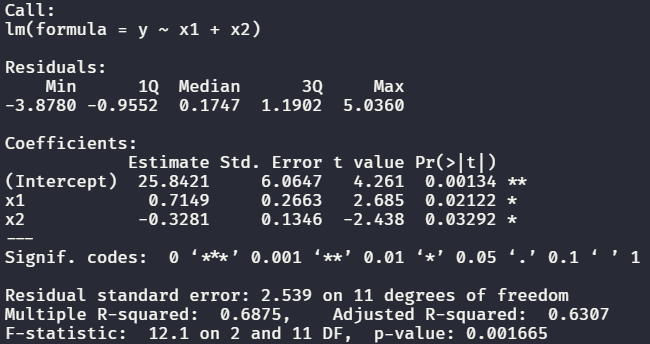
\includegraphics[width=0.7\linewidth]{bai-3-5-model-1}
		\caption{Tham số mô hình \ref{model:12}}
		\label{fig:bai-3-5-model-1}
	\end{figure}
	
	Hệ số hồi quy:
	\[\hat{\beta_0}=25.84214, \hat{\beta_1}=0.7148959, \hat{\beta_2}=-0.3281129\]
	
	\item Mô hình \ref{model:13}
	\begin{figure}[h]
		\centering
		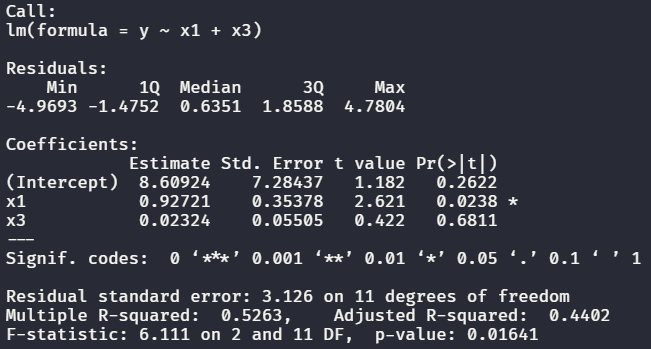
\includegraphics[width=0.7\linewidth]{bai-3-5-model-2}
		\caption{Tham số mô hình \ref{model:13}}
		\label{fig:bai-3-5-model-2}
	\end{figure}
	
	Hệ số hồi quy:
	\[\hat{\beta_0'}=8.609241, \hat{\beta_1'}=0.9272087, \hat{\beta_3'}=0.02323681\]
	
	\item Mô hình \ref{model:23}
	\begin{figure}[h]
		\centering
		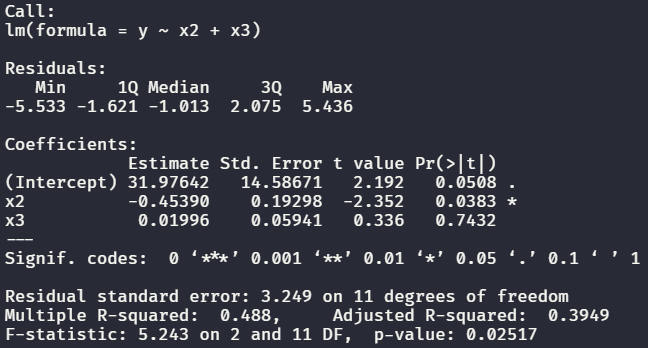
\includegraphics[width=0.7\linewidth]{bai-3-5-model-3}
		\caption{Tham số mô hình \ref{model:23}}
		\label{fig:bai-3-5-model-3}
	\end{figure}

	Hệ số hồi quy:
	\[\hat{\beta_0''}=31.97642, \hat{\beta_2''}=-0.4538954, \hat{\beta_3''}=0.01996295\]
\end{itemize}

\subsubsection*{3. Với độ tin cậy 95\%, tìm khoảng tin cậy cho các tham số trong mô hình với 2 biến độc lập $x_1$ và $x_2$.}
Viết lại mô hình: $Y = \beta_0 + \beta_1 X_1 + \beta_2 X_2 + \epsilon$

\begin{center}
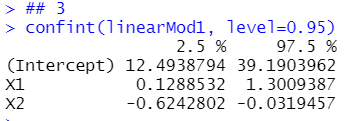
\includegraphics{bai3_3.PNG} 
\end{center}

Dựa vào kết quả mô hình, với độ tin cậy 95\%, khoảng tin cậy của:

\begin{itemize}
    \item $\beta_0$ là $[12.4939, 39.1904]$
    \item $\beta_1$ là $[0.1289, 1.3009]$
    \item $\beta_2$ là $[-0.6243, -0.0319]$
\end{itemize}

\subsubsection*{4. Xác định hệ số xác định cho mỗi mô hình trong câu 1.}

\begin{itemize}
	\item Mô hình \ref{model:12} có bảng ANOVA:
	\begin{figure}[h]
		\centering
		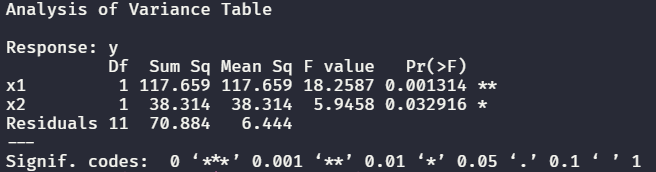
\includegraphics[width=0.7\linewidth]{bai-3-5-anova-1}
		\caption{Bảng ANOVA của mô hình \ref{model:12}}
		\label{fig:bai-3-5-anova-1}
	\end{figure}
	
	Hệ số xác định:
	\[R^2 = \dfrac{SSR}{SST} = 0.6875395\]
	
	\item Mô hình \ref{model:13} có bảng ANOVA:
	\begin{figure}[h]
		\centering
		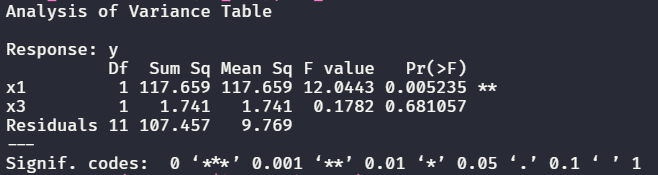
\includegraphics[width=0.7\linewidth]{bai-3-5-anova-2}
		\caption{Bảng ANOVA của mô hình \ref{model:13}}
		\label{fig:bai-3-5-anova-2}
	\end{figure}
	
	Hệ số xác định:
	\[R'^2 = \dfrac{SSR}{SST} = 0.5263211\]
	
	\item Mô hình \ref{model:23} có bảng ANOVA:
	\begin{figure}[h]
		\centering
		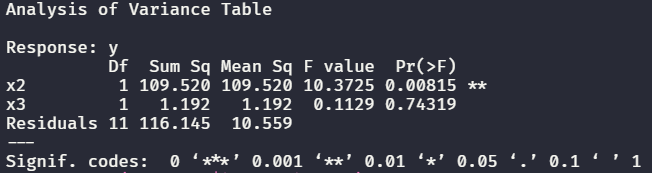
\includegraphics[width=0.7\linewidth]{bai-3-5-anova-3}
		\caption{Bảng ANOVA của mô hình \ref{model:23}}
		\label{fig:bai-3-5-anova-3}
	\end{figure}
	
	Hệ số xác định:
	\[R''^2 = \dfrac{SSR}{SST} = 0.4880253\]
\end{itemize}


\subsubsection*{5. Trong các mô hình trên, mô hình nào thích hợp nhất để giải thích sự biến thiên của $Y$ ?}

Do các mô hình đều có cùng số lượng biến độc lập, ta so sánh hệ số xác định ($R^2$) để xét xem mô hình nào thích hợp nhất. Với kết quả từ câu 4, ta có được thứ tự tăng dần các hệ số xác định từ các mô hình của $Y$ là \[R''^2 < R'^2 < R^2 \]

Vậy với hệ số $R^2$ cao nhất thì mô hình hai biến độc lập $x_1, x_2$ là phù hợp nhất để giải thích sự biến thiên của $Y$.

\subsubsection*{6. Viết mô hình tuyến tính dưới dạng ma trận với số biến độc lập nhiều nhất có thể, và xác định kích thước của ma trận.}

Giả thiết cho mô hình $\mathbf{Y} = \mathbf{X}\beta + \epsilon$:
\begin{itemize}
	\item Tập dữ liệu trong mô hình không xảy ra hiện tượng đa cộng tuyến.
	\item $\epsilon$ thuộc phân phối chuẩn với độ lệch chuẩn vector $0$ và phương sai $\sigma^2$.
\end{itemize}

Dựa vào dữ liệu đề bài, số biến độc lập nhiều nhất có thể là 3 biến $(X_1,X_2,X_3)$:

\[{Y_{14 \times 1}} = \left[ {\begin{array}{*{20}{c}}
  {{y_1}} \\ 
   \vdots  \\ 
  {{y_{14}}} 
\end{array}} \right];{X_{14 \times 4}} = \left[ {\begin{array}{*{20}{c}}
  1&{{x_{1,1}}}&{{x_{1,2}}}&{{x_{1,3}}} \\ 
  \vdots & \vdots & \vdots & \vdots  \\ 
  1&{{x_{14,1}}}&{{x_{14,2}}}&{{x_{14,3}}} 
\end{array}} \right];{\beta _{4 \times 1}} = \left[ {\begin{array}{*{20}{c}}
  {{\beta _0}} \\ 
   \vdots  \\ 
  {{\beta _3}} 
\end{array}} \right];{\varepsilon _{14 \times 1}} = \left[ {\begin{array}{*{20}{c}}
  {{\varepsilon _1}} \\ 
   \vdots  \\ 
  {{\varepsilon _{14}}} 
\end{array}} \right]\]

Với dữ liệu đề bài, một số dòng đầu và dòng cuối của ma trận $\mathbf{X}$ và vec-tơ $\mathbf{Y}$ là:

\[{Y_{14 \times 1}} = \left[ {\begin{array}{*{20}{c}}
  {{12}} \\
  {{14}}  \\
   \vdots  \\ 
  {{25}} \\
  {{21}}
\end{array}} \right];{X_{14 \times 4}} = \left[ {\begin{array}{*{20}{c}}
  1&{{2}}&{{45}}&{{121}} \\ 
  1&{{1}}&{{43}}&{{132}} \\ 
  \vdots & \vdots & \vdots & \vdots  \\ 
  1&{{12}}&{{35}}&{{174}} \\ 
  1&{{7}}&{{29}}&{{180}} 
\end{array}} \right]\]

\subsubsection*{7. Ước lượng các hệ số hồi quy trong mô hình tuyến tính ở câu 6.}
Viết lại mô hình: $Y = \beta_0 + \beta_1 X_1 + \beta_2 X_2 + \beta_3 X_3 + \epsilon$

\begin{center}
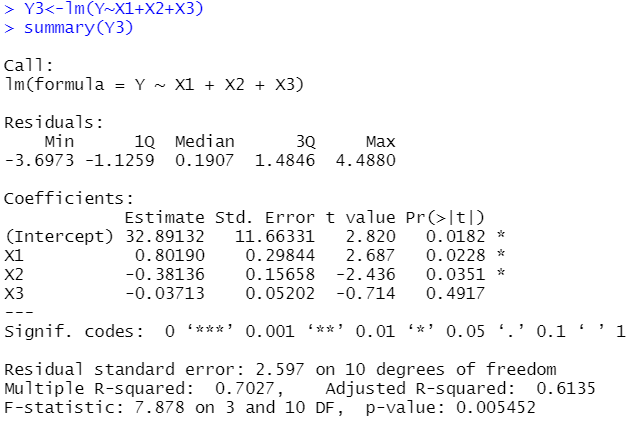
\includegraphics{bai3_6.PNG} 
\end{center}
Dựa vào kết quả mô hình, ta có các hệ số hồi quy:
$$\hat{\beta_0} = 32.89132, \hat{\beta_1} = 0.8019, \hat{\beta_2} = -0.38136, \hat{\beta_3} = -0.03713$$
\subsubsection*{8. Trong mô hình tuyến tính ở câu 6, tính ước lượng của $\mathbb{V}(\epsilon)$ và $\mathbb{V}(\hat{\beta})$.}

\textbf{(a)} Ước lượng phương sai của sai số, $\mathbb{V}(\epsilon)$. Ta có  $\mathbb{V}(\epsilon) = \mathbf{I}_{14}\sigma^2$

Với $\sigma^2$ được ước lượng bởi 
$$\hat{\sigma}^2 = MSE = \displaystyle \frac{SSE}{n-4} = 6.745$$

Vậy ước lượng của  $\mathbb{V}(\epsilon)$ là 
\begin{center}
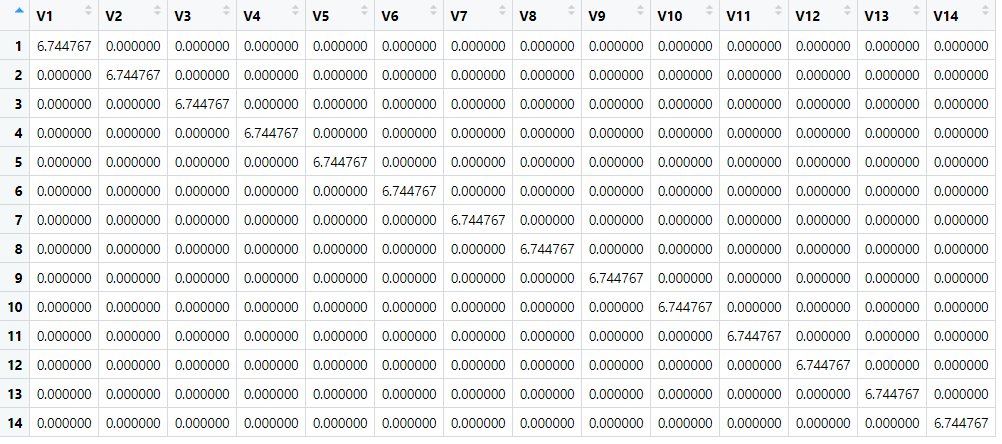
\includegraphics[scale = 0.8]{bai3_8a.PNG} 
\end{center}

\textbf{(b)} Ước lượng phương sai của $\hat{\beta}$:

\[\mathbb{V}(\hat{\beta}) = \left[ {\begin{array}{*{20}{c}}
  var(\hat{\beta_0}) \\
  var(\hat{\beta_1})  \\
   var(\hat{\beta_2})\\
 var(\hat{\beta_3})
\end{array}} \right]  = \left[ {\begin{array}{*{20}{c}}
  \mathbf{Se}^2(\hat{\beta_0}) \\
  \mathbf{Se}^2(\hat{\beta_1})  \\
   \mathbf{Se}^2(\hat{\beta_2})\\
 \mathbf{Se}^2(\hat{\beta_3})
\end{array}} \right]\]

Cách khác: 

\begin{center}
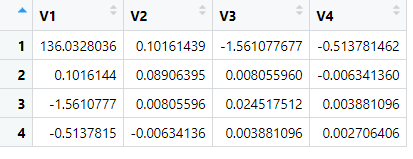
\includegraphics{bai3_8b.PNG} 
\end{center}

\subsubsection*{9. Với độ tin cậy 95\%, tìm khoảng tin cậy cho $\mathbb{V}(\epsilon)$. }

\begin{center}
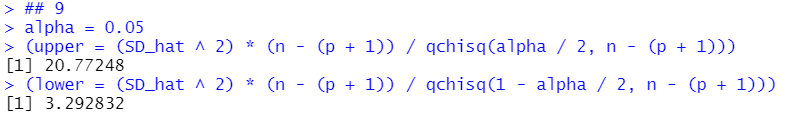
\includegraphics{bai3_9.PNG} 
\end{center}

Với độ tin cậy 95\%, khoảng tin cậy của $\hat{\sigma}^2$ là $\left(3.292832;20.77248\right)$

\subsubsection*{10. Khi thêm 2 biến độc lập $x_3$ và $x_2$ vào mô hình chỉ với 1 biến độc lập $x_1$ thì làm cho chất lượng ước lượng cao hơn không?}

Để kiểm tra chất lượng ước lượng, trước tiên, ta lần lượt kiểm định các giả thuyết sau:
\begin{enumerate}[label=(\roman*)]
	\item $H_0: \beta_1 = 0$ cho mô hình $Y = \beta_0 + \beta_1X_1 + \epsilon$
	
	Đặt giả thuyết kiểm định:
	\[\begin{cases}
		H_0 : \beta_1 = 0\\
		H_1 : \beta_1 \ne 0
	\end{cases}\]

	Kết quả mô hình chỉ với 1 biến độc lập $X_1$
	\begin{center}
		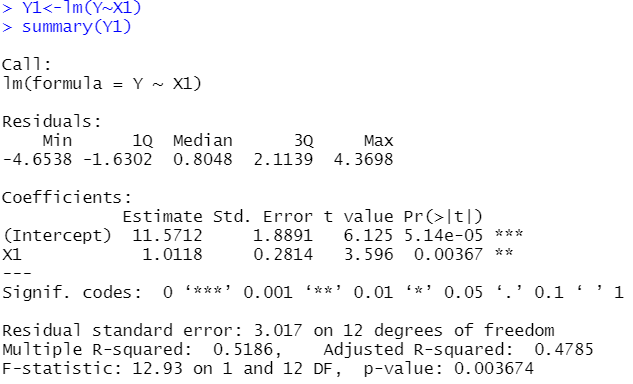
\includegraphics{bai3_10.PNG} 
	\end{center}
	
	Từ đó, ta có $p\_value = 0.00367 < \alpha = 0.05$, suy ra bác bỏ $H_0$ với mức ý nghĩa 5\%, nghĩa là $Y$ được giải thích bởi $X_1$.
	
	\item $H_0: \beta_2 = 0$ cho mô hình $Y = \beta_0 + \beta_1X_1 + \beta_2X_2 + \epsilon$
	
	Đặt giả thuyết kiểm định:
	\[\begin{cases}
		H_0 : \beta_2 = 0 \text{ hay } Y = \beta_0 + \beta_1 X_1 + \epsilon \\
		H_1 : \beta_2 \ne 0 \text{ hay } Y = \beta_0 + \beta_1 X_1 + \beta_2 X_2 + \epsilon
	\end{cases}\]
	
	Thực hiện kiểm định Fisher từng phần, ta có thống kê của kiểm định: 
	$$F = \displaystyle \frac{\left [ SSE (H_0) - SSE(H_1) \right ] / r}{SSE(H_1)/(n-p)} \sim F_{(r,n-p)} \text{ khi } H_0 \text{ đúng},$$
	trong đó $r = 1, n = 14, p = 3$.
	
	Trước tiên, ta cần tính $SSE (H_0)$ và $SSE(H_1)$, với $SST = 226.857$ từ câu 4:
	$$SSE(H_0) = SST - SSR_{x_1} = 109.195 \text{, (đặt là } SSE_{x_1})$$
	$$SSE(H_1) = SST - SSR_{x_1} - SSR_{x_2|x_1} = 70.881 \text{, (đặt là }  SSE_{x_1,x_2})$$
	
	Giá trị thống kê $$F_{obs} = 5.946$$
	
	Với mức ý nghĩa $\alpha = 0.05$, tra bảng Fisher ta được:
	$$F_{1-\alpha}(r,n-p) = F_{0.95}(1,11) = 4.8443$$
	
	Vì $F_{obs}>F_{0.95}(1,11)$ nên ta bác bỏ $H_0$ với mức ý nghĩa 5\%, nghĩa là $Y$ được giải thích bởi $X_1,X_2$.
	
	\item $H_0: \beta_3 = 0$ cho mô hình $Y = \beta_0 + \beta_1X_1 + \beta_2X_2 + \beta_3X_3 + \epsilon$
	
	Đặt giả thuyết kiểm định:
	\[\begin{cases}
		H_0 : \beta_3 = 0 \text{ hay } Y = \beta_0 + \beta_1 X_1 + \beta_2 X_2 + \epsilon \\
		H_1 : \beta_3 \ne 0 \text{ hay } Y = \beta_0 + \beta_1 X_1 + \beta_2 X_2 + \beta_3 X_3 + \epsilon 
	\end{cases}\]

	Thực hiện kiểm định Fisher từng phần, ta có thống kê của kiểm định: 
	$$F = \displaystyle \frac{\left [ SSE (H_0) - SSE(H_1) \right ] / r}{SSE(H_1)/(n-p)} \sim F_{(r,n-p)} \text{ khi } H_0 \text{ đúng},$$
	trong đó $r = 1, n = 14, p = 4$.
	
	Trước tiên, ta cần tính $SSE (H_0)$ và $SSE(H_1)$:
	$$SSE(H_0) = SST - SSR_{x_1} - SSR_{x_2} = 70.881 \text{, (đặt là }  SSE_{x_1,x_2}) $$
	$$SSE(H_1) = SST - SSR_{x_1} - SSR_{x_2} - SSR_{x_3} = 69.14 \text{, (đặt là }  SSE_{x_1,x_2,x_3})$$
	
	Giá trị thống kê $$F_{obs} = 0.2518$$
	
	Với mức ý nghĩa $\alpha = 0.05$, tra bảng Fisher ta được:
	$$F_{1-\alpha}(r,n-p) = F_{0.95}(1,10) = 4.9646$$
	
	Vì $F_{obs}<F_{0.95}(1,10)$, suy ra chưa đủ cơ sở để bác bỏ $H_0$ với mức ý nghĩa 5\%, nghĩa là $Y$ chưa được giải thích bởi $X_3$.
\end{enumerate}

\textbf{\underline{Kết luận:}}

Qua kiểm định các giả thuyết trên, vì $Y$ chưa được giải thích bởi $X_3$ mà chỉ có thể được giải thích bởi $X_1, X_2$, nên ta có kết luận như sau:
\begin{itemize}
	\item Khi thêm biến độc lập $X_2$ vào mô hình $X_1$, do thực hiện trên cùng mẫu, số lượng biến độc lập khác nhau, ta so sánh giá trị $R^2$ hiệu chỉnh. Nhận thấy:
	
	\[R^2_{adj_1} = 0.4785 < R^2_{adj_2} = 0.6307\]
	
	Vậy khi thêm $X_2$ vào mô hình với một biến độc lập $X_1$ thì chất lượng ước lượng sẽ được cải thiện.
	
	\item Khi thêm biến độc lập $X_3$ vào mô hình $X_1,X_2$ sẽ không cải thiện được chất lượng ước lượng;
\end{itemize}

\end{document}
